\chapter{Introduction}
\label{chapter:introduction}

There are systems where the number of elements that conform it is considerably
low or it is easy to understand how the elements interact among them. For
example, analyzing projectile trajectories is a rather easy to understand
problem, where the number of significant factors involved in the problem is
low. As another example, we can perform a structural analysis of a building, and
even though the number of loads being involved in the analysis can be very high,
one can still understand how the loads are going to interact among them with a
% This is true, but this  possible because of how the system is modeled,
% ignoring the many variables involved. For instance, tiny air waves or changes in steel beams. 
% Never the less these systems are easy to model and are usefull at a certain level of abstraction.
% Maybe you could briefly comment on this.  - Mario
very high precision. It is worth mentioning that these models provide a
simplification of the problem they are modeling; they do not consider variables
that are not significant to the problem of interest. In contrast, there are
systems where the significant elements that are interacting in it are very hard
to understand or the number of elements is very high. For example, understanding
why human beings can change their religious beliefs is a situation which is very
hard to understand, or to calculate what is going to be the final position of
thousands of paper sheets thrown in the air at the same time is a task which is
almost impossible to do. These systems that are hard to model by simple
mathematical formulas are known as complex systems \cite{Anderson1999}. % Add a reference to an important paper on CS.

A financial market is an example of a complex system, where thousands of traders
are constantly deciding how many units are going to be sold or bought at
arbitrary intervals of time. The strategies followed by each of these traders
can vary from technical analysis using mathematical formulas to basing their
decision on news interpretations. And even after establishing a trading
strategy, traders can decide to ignore their conclusions due to subjective
factors such as ``having a bad feeling about this.'' As a consequence, financial
markets are frequently used to showcase complexity theory concepts
\cite{Arthur1999} \cite{Bundesbank2007}. Even though these markets can exhibit an
almost chaotic behavior, certain patterns still emerge, which stop financial
markets from being labeled as chaotic systems \cite{Castillo2001}.

One of the methods used for forecasting how a financial market will behave in
price is to use fundamental analysis \cite{Kadiri2015}. This type of analysis takes into % Reference missing
account knowledge that you can gather from the factors that influence the % Can we say knowledge instead of information?
market's price. For example, if a company releases their financial statements
and they demonstrate that the company is performing financially well, it is very
likely that a surge in the company's stock price will occur. In this case, a
number of traders will become aware of this information and will decide to buy
the company's stock.

In contrast to fundamental analysis, technical analysis can be used to forecast
the behavior of a market. Technical analysis is conformed by any process that
forecasts price movements where only data related to past and current prices of
a financial market is involved. For example, a traditional technique is to use
moving averages to obtain a price which is representative of the past $N$
prices. In technical analysis it is common to chart these methods -- which are
called technical indicators -- along with the real prices of a financial market,
as can be seen in Figure \ref{figure:moving-average-example}. This way a trader
can see all the information in a graphical manner, and have everything plotted
on a single chart.

\begin{figure}
  \caption{Moving average example} \centering
  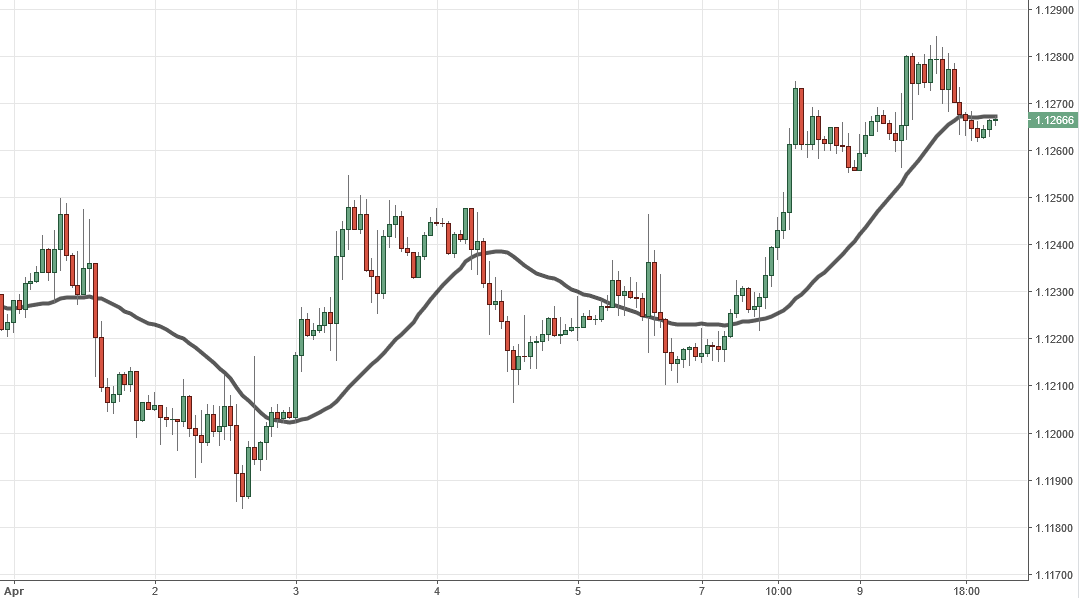
\includegraphics[width=0.7\textwidth]{img/moving-average.png}
  \label{figure:moving-average-example}
\end{figure}

Some researchers believe that technical analysis works because it falls under
the category of a self-fulfilling prophecy \cite{Salganik2008}: it works
because many people use it. If enough people buy an asset because technical
analysis predicts that it is a good idea to do so, the price will rise and then
technical analysis is correct. Nevertheless, there is a big number of technical
indicators, and many of these technical indicators are parametrized, which means
that there are many possible ways of interpreting a market using technical
indicators. Still, there is enough empirical evidence that demonstrates that
technical analysis can help a trader to better understand a market
\cite{Achelis2000} \cite{Fund1992} \cite{Li1999}. 
%% Are there any references about this empirical evidence? or is it anecdotal?
A possible
explanation behind this is that, although there are virtually an infinite number
of possible configurations that a technical indicator can adopt, not all of them
seem to ``follow the market,'' i.e. a technical indicator needs to be configured
to match the behavior of past prices, and not simply use an arbitrary
configuration. This further reinforces the self-fulfilling prophecy hypothesis
behind technical analysis: the traders that are creating the price movements in
a market are using technical indicators that are being adjusted to the price
that they created themselves.

Taking into consideration the discussion in the previous paragraph, technical
indicators thus work by trying to find a pattern in the price movements. These
patterns are then interpreted in some way by traders, and inferences about the
market are created, such as: ``this market is presenting a high volatility'' or
``this market is going uptrend.'' This also implies that technical indicators can
be interpreted in different ways, depending on the trader's knowledge and
opinion.

In conclusion, in order to understand a market from a technical analysis point
of view, one needs to take into consideration that a number of traders with
different ideas and different interpretations of the market are creating the
price movements. Forecasting or modelling tools taking a technical analysis
approach should take into consideration these factors. %% This thesis work proposes
%% that the problem of modelling these traders can be solved by using a multi-agent
%% system where technical analysis is used to describe how the agents are
%% perceiving the market.

% There is a bridge missing over here. Please write a conclusion paragraph 
% for this passage. Briefly state what is the problem and what could be a soulution?
% - Mario 

%% P.D., after reading further, I think the section break could be the problem.
%% Move it to the point where you are going to state the structure or even
%% remove it

%% \section{Thesis Structure}
%% \label{section:thesis-structure}

This thesis work proposes that the problem of modelling these traders can be
solved by using a multi-agent system where technical analysis is used to
describe how the agents are perceiving the market. In the end, the methodology
presented in this work can be used as an approach to analyze and interpret a
financial market to obtain insights that can be used to describe the behavior
behind that market and create a trading
% and create a profitable trading  -> and create a trading strategy with better perfomance 
% or something like this. We cannot warrant a profitable trading strategy. 
strategy that can help a trader take better trading decisions. In this first
Chapter the reader finds the motivation of this work, such as why understanding
a financial market is a problem and why solving this problem is beneficial (see
Section \ref{section:justification}).

% In the first sentence ``propose a novel series of approaches to how a financial
% market can be interpreted and analyzed''

% the things you approach ``interpreted and analyzed'' are to far away, maybe:
% ... approaches on how to analize and interpret a financial market ...  % we
% must try not to use words such as ``great importance'' change to? `` %
% ... solving this problem is beneficial''.

The proposed method in this document is based on at least three different
fields, which are computational intelligence, complexity theory and financial
markets. Chapter \ref{chapter:preliminaries} is dedicated to explaining the
concepts related to these fields, which are needed to understand the contents of
the following Chapters and the thesis overall.

% Depending on space the comment on the background of readers could be deleted.

Once the reader is acquainted with the necessary terminology, concepts and ideas
discussed in the aforementioned Chapter, a series of related works are presented
in Chapter \ref{chapter:related-work}. These works help the reader to further
understand the problem being solved in this thesis, as one can see how different
approaches have been taken in the past to solve similar problems. Also, the
presented related works indirectly fuel the justification of this thesis, as the
reader can realize how similar approaches to the proposed method have improved
other fields of research.

The actual proposed method of this thesis is presented in Chapter
\ref{chapter:proposed-method}. In this Chapter the reader can find how the
problem discussed in this introduction can be
solved. Additionally, some other proposals are discussed, such as how
intuitionistic fuzzy sets and systems can be used to represent a knowledge in an
expanded way, in contrast to traditional fuzzy sets and systems.

A particular implementation of the proposed method is discussed in Chapter
\ref{chapter:implementation}, which covers some technical details, such as what
programming languages were used and how exactly the ideas from Chapter
\ref{chapter:proposed-method} were programmed. As each of the concepts discussed
in Chapter \ref{chapter:proposed-method} are covered in the implementation, some
of the Sections from both Chapters match in name.

After having implemented the proposed method, a series of experiments were
performed to demonstrate how it compares to other similar solutions. The
experiments also help the reader to understand how the method can be used to
obtain insights from a financial market, as well as how one can use these
insights to perform better decisions while trading in such markets. These % trading IN such markets? or is jargon?
experiments are presented in Chapter \ref{chapter:experiments-and-results}, where their
design is discussed, and the results obtained from the experiments are also presented.

Lastly, the reader can find some conclusions about the work developed for this
thesis in Chapter \ref{chapter:conclusions-and-future-work}, as well as various propositions on
how the present work could be further developed in the future.

\section{Justification}
\label{section:justification}

Understanding the nature of financial markets is of utter importance, as
financial markets play a big role in the economy system of any country. Having
several tools to understand financial markets can help to forecast financial
crises, understand the development of the economy of a company, and take better
decisions when investing.

The problem stated at the beginning of this Chapter can be
broken into the following pieces: a forecasting or modelling solution needs to
consider 1) a number of traders manipulating the price movement in a financial
market, 2) each of these traders have different opinions about how to trade a
market depending on how the market is behaving, and 3) each of these traders
interpret the market differently.

Traders can be seen as agents in a multi-agent system, where each of these
agents receive data from another agent: a broker. The broker is in charge of
sending the price information about a financial market to every trader. This
data can be used later as the input for all the technical indicators. The agents
representing the traders never interact among them, only with the broker. In
addition to receiving the financial market data from the broker, a trader can
also send transaction operations to the broker, such as buy or sell orders. Many
authors consider multi-agent systems and agent-based models as one of the better
tools for modelling and simulating financial markets \cite{Lebaron2001}
\cite{Gamil2007} \cite{Boer-Sorban2008} \cite{Suarez2008} \cite{Suarez2012}, due
to their flexibility to represent very complex systems. % Also there is the
paper from Puga, please add a reference.

Implementing an agent-based solution allows not only to simulate the actions
that different entities can take in a complex system, but also to model how the
agents are perceiving their environment and the inference process used to take
such actions. This is interesting because the simulated models created using an
agent-based solution can then be examined by looking at how each of the agents
behaves in the system.

In addition to the use of a multi-agent architecture to simulate the traders,
the actions of the traders are modelled by the use of fuzzy systems. These
systems allow the system to increase its interpretability: why a trader took
certain decision can be understood after examining the composition of the fuzzy
rules. Specifically, this work uses intuitionistic fuzzy systems in order to
provide another layer of interpretation, as this type of systems can explain the
hesitancy that is present in the inputs and outputs of the systems.

The agents' perception of their environment is determined through the use of
technical analysis, which is used to provide a simplified version of the price
data of a financial market. The preprocessing algorithms (technical indicators)
are parameterized, which means that can be adjusted according to an agent's
profile (beliefs).

In the end, the presented method provides an architecture that can successfully
model and describe the interaction among the different traders that create the
price increments and decrements in a financial market.

%% Then talk about how to model the agents' actions or belfies, etc.

%% We can justify two things: why the problem is important and why the
% method works

%% why multi-agent, why intuitionistic, why retracements
